\documentclass[12pt,a4paper]{article}
\pdfoutput=1

\usepackage[utf8]{inputenc}
\usepackage[T1]{fontenc}
\usepackage[swedish]{babel}
\usepackage{amsmath}
\usepackage{lmodern}
\usepackage{listings}
\usepackage{units}
\usepackage{icomma}
\usepackage{color}
\usepackage{graphicx}
\usepackage{multicol,caption}
\usepackage{bbm}
\usepackage{hyperref}
\usepackage{xfrac}
\newcommand{\N}{\ensuremath{\mathbbm{N}}}
\newcommand{\Z}{\ensuremath{\mathbbm{Z}}}
\newcommand{\Q}{\ensuremath{\mathbbm{Q}}}
\newcommand{\R}{\ensuremath{\mathbbm{R}}}
\newcommand{\C}{\ensuremath{\mathbbm{C}}}
\newcommand{\rd}{\ensuremath{\mathrm{d}}}
\newcommand{\id}{\ensuremath{\,\rd}}
\newenvironment{Figure}
  {\par\medskip\noindent\minipage{\linewidth}}
  {\endminipage\par\medskip}
\newcommand{\HRule}{\rule{\linewidth}{0.5mm}}

\renewcommand{\lstlistingname}{Programkod}

\definecolor{mygreen}{RGB}{28,172,0}
\definecolor{mylilas}{RGB}{170,55,241}

\lstset{language=Matlab,%
  %basicstyle=\color{red},
  breaklines=true,%
  morekeywords={matlab2tikz},
  keywordstyle=\color{blue},%
  morekeywords=[2]{1}, keywordstyle=[2]{\color{black}},
  identifierstyle=\color{black},%
  stringstyle=\color{mylilas},
  commentstyle=\color{mygreen},%
  showstringspaces=false,%without this there will be a symbol in the places where there is a space
  numbers=left,%
  frame=single,
  numberstyle={\tiny \color{black}},% size of the numbers
  numbersep=9pt, % this defines how far the numbers are from the text
  emph=[1]{for,end,break},emphstyle=[1]\color{red}, %some words to emphasise
  %emph=[2]{word1,word2}, emphstyle=[2]{style},
}

\begin{document}

\title{Vocol harum}
\author{A. Lundin, E. Sandrén, K. Eskilson}
\date{\today}

\begin{titlepage}
\begin{center}

% Title
{ \huge  Vocol Harum \\[0.4cm] }

\large Generering av harmonisk treklang

\HRule \\[1.5cm]

A. Lundin
\emph{alilu684},
E. Sandrén
\emph{erila135},
K. Eskilson
\emph{klaes950}\\[1.5cm]

TFYA65 – Ljudfysik

\vfill

% Bottom of the page
{\large \today}

\end{center}
\end{titlepage}


% empty page
\newpage\null\thispagestyle{empty}\pagenumbering{gobble}\newpage

\newpage\pagenumbering{arabic}% Arabic page numbers (and reset to 1)

\renewcommand{\abstractname}{Sammanfattning}
\begin{abstract}
  Denna rapport redogör för ett projektarbete gjort i kursen TFYA65 – Ljudfysik. Projektets syfte är att med hjälp av fysikaliska modeller samt tillämpningar lära sig mer inom ljud- och signalbehandling.
\end{abstract}

\newpage

\tableofcontents

\newpage

\section{Bakgrund}

Projektets mål är att skapa en så kallad vocal harmonizer. Detta innebär ett program som lägger en ters och en kvint ovanpå en ton, och därigenom skapar en treklang på den ton som mottages av programmet.

\subsection{Diatoniska intervall}

Hädan efter krävs en förståelse för vad en skala innebär, och vad diatoniska intervall är.

Ters och kvint är förhöjningar av frekvensnivån utav grundtonen enligt \emph{tabell \ref{table:diatonic}}. För att nå kvint/ters behöver alltså originalljudets frekvens höjas. Då dessa värden är helt oberoende av ton är det irrelevant att ta reda på grundtonens egna frekvens för att göra frekvenshöjningen \cite{bib:schmidt}. Enbart en av liten och stor ters är aktuell i en skala, och hädanefter kommer den stora tersen att användas. \\

\begin{table}[h]
  \begin{center}
    \begin{tabular}{l l l}
      Diatoniskt intervall & Frekvensfaktor & Exempel (hz) \\
      \hline
      Grundton & 1 & 440 \\
      Liten ters (moll) & 1.2 & 528 \\
      Stor ters (dur) & 1.25 & 550 \\
      Kvint (dur och moll) & 1.5 & 660 \\
    \end{tabular}
    \caption[Table caption text]{Diatoniska intervall}
    \label{table:diatonic}
  \end{center}
\end{table}

\section{Metod}
Samtliga medlemmar i gruppen började arbetet med att läsa på om signalbehandling och tidigare experiment som gjorts inom området. Arbetet delades sedan upp i mindre projekt som sammanfördes och utvärderades i slutet av varje arbetspass, och det bestämdes vad som kunde sparas och inte.

Det verktyg som använts främst i projektet är MATLAB. För inspelning och uppspelning användes datorns inbyggda hårdvarukomponenter.

Ett program skapades som läser in en signal och gör om den till frekvensdomän med hjälp av inbyggda transformfunktioner i MATLAB. Det görs då ljudets fasgång inte går att förändra i tidsdomänen. Programmet delar upp ljudet i mindre segment där brus reduceras, och fasgången studeras. Skillnaden i fasgång mellan nuvarande segment och förgående beräknas \cite[kapitel 7.4]{bib:dafx}. Genom denna skillnad kan en syntetisk fasgång skapas. Den syntetiska fasgången måste användas för att undvika att ett fasfel uppstår vid omsamplingen \cite{bib:moinet}. Signalen transformeras sedan tillbaka till tidsdomänen med hjälp av invers fouriertransform, se \emph{programkod \ref{lst:fft}}. Segmentet samplas om i tidsdomänen genom att samplingsvärden med visst intervall raderas. Intervallet är relativt till vald tonhöjning. En linjär interpolation sker av kvarstående samplingsvärden för att ljudet skall vara kontinuerligt. De nya tonerna, kvinten och tersen, kan sedan adderas med grundtonen i tidsdomänen.

\begin{lstlisting}[caption={fouriertransform (fft) samt invers fouriertransform (ifft)},label={lst:fft}]
  f         = fft(fftshift(grain));
  r         = abs(f);
  meanValue = mean(r);
  threshold = meanValue*1.1;
  r(r < threshold) = 0;
  grain = fftshift(real(ifft(f)));
\end{lstlisting}

För att reducera brus görs åtgärder på två sätt. Medelvärdet av frekvensamplituden i varje segment beräknas och multipliceras med 1,1. Detta värde verkar som tröskelvärde, och alla frekvenser inom tidsintervallet med amplitud lägre än tröskelvärdet filtreras bort. Detta fungerar bra i de segment där någon ton är dominant, men vid inspelning med pauser (exempelvis en inspelning av sång) kommer vissa segment ha medelintensitet som är för låg för att verka som tröskelvärde. Det skulle resultera i att bruset reduceras då en stark ton spelas och sedan förstärks vid tystnad.

Den andra åtgärden kontrollerar därför medelvärdet av ljudintensiteten i varje segment. Är detta värde lägre än 30dB modifieras inget ljud alls och programmet går vidare till nästa segment.

För att höja frekvensen på ett ljud flyttas de sampelpunkter som verkar på originalsignalen isär med en önskad faktor. De trycks sedan ihop till ursprungligt avstånd och signalen “följer med”, se \emph{figur \ref{fig:resample}}. På så sätt fås ett tidsfel som beror på faktorn för samplingen, det vill säga den grad som frekvensen ska höjas. Under uppspelning av ljud blir därför kvintens ljud något kortare än originalet och tersen ännu kortare. En lösning på problemet är repetition och överlappning \cite{bib:tfya}. Signalen delas upp i hanningfönster. För att förlänga signalen repeteras skärningsdelen av angränsande segment, se \emph{figur \ref{fig:overlap}}. Det ger visserligen ett fel, men om segmenten är tillräckligt små och repetitionsdelen liten kommer detta inte att höras.

\begin{Figure}
  \centering
    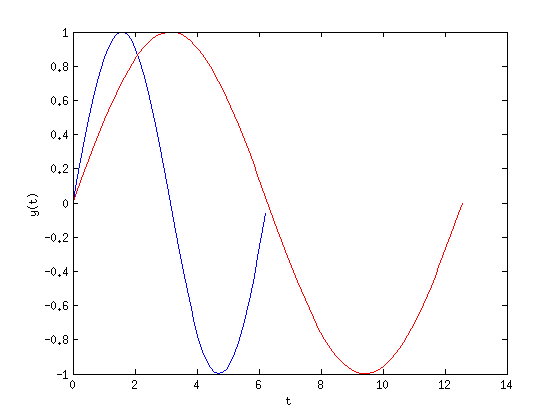
\includegraphics[width=0.7\linewidth]{./images/resample.png}
    \captionof{figure}{\emph{Godtycklig sinussignal i tidsdomänen. Originalsignalen (röd) har förhöjts till dubbla frekvensen och därmed tryckts ihop (blå).}\label{fig:resample}}
\end{Figure}

\begin{Figure}
  \centering
    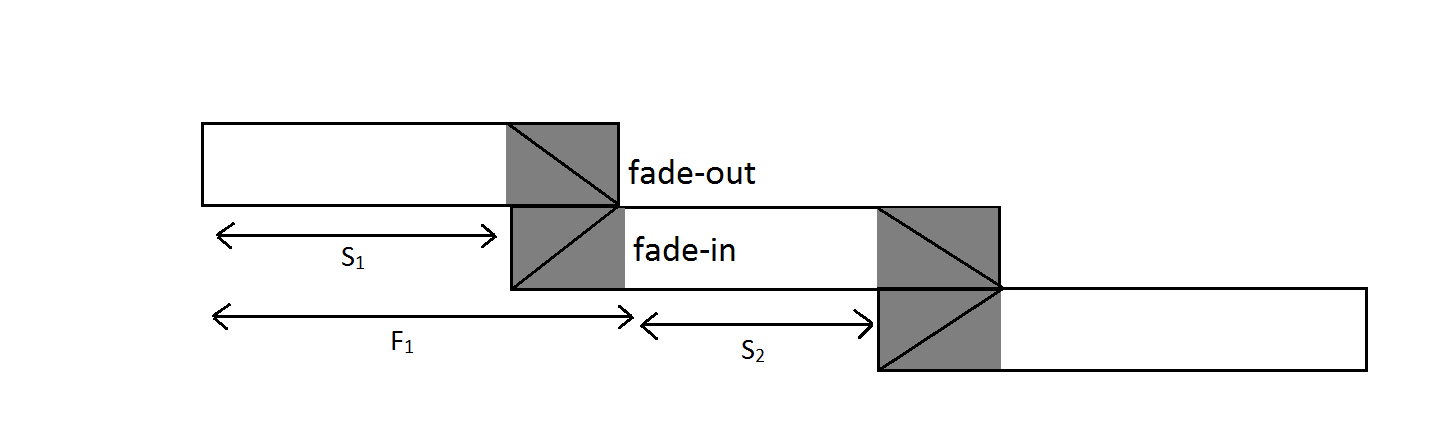
\includegraphics[width=0.7\linewidth]{./images/overlap.png}
    \captionof{figure}{\emph{Överlappning av fönster, F, gör att mellanrummet mellan segment S1 och S2 ökas.}\label{fig:overlap}}
\end{Figure}

En metod för att använda funktionen i realtid gjordes till sist genom att dela upp inspelningen i korta intervall om cirka en halv sekund. Då programmet spelat in ljud från ett tidsintervall får det genast genomgå transformation och spelas sedan upp i högtalaren samtidigt som nästa tidsintervall spelas in. För att simulera realtid görs sampeltiden liten.

\section{Resultat}

Det slutgiltiga resultatet är en MATLAB-funktion som behandlar ett förinspelat ljudstycke. Ljudet läses och delas upp i segment på 512 sampels. Dessa segment studeras i hanningfönstren på 2048 samples. Ljudintensiteten i varje segment kontrolleras mot ett tröskelvärde och om det överstiger värdet transformeras ljudsegmentet om till frekvensdomänen med Fouriertransform. Brus reduceras och en fasgenerering görs. Signalen transformeras tillbaka med invers Fouriertransform. Frekvensen samplas sedan om med rätt faktor för att skapa ters och kvint. De nya tonerna adderas till originaltonen, och nästa segment behandlas. Om intensiteten inte överskrider tröskelvärdet förblir segmentets värden oförändrade, och programmet går vidare till nästa segment. Då samtliga tidsintervall transformerats och omsamplats spelas den nya melodin upp.

\section{Diskussion}

I och med att MATLAB ej är gjort för snabb och effektiv beräkning i realtid inleddes arbetet med att göra ett program i Python. Fördelen mot MATLAB är att Python effektivt utnyttjar moderna datorers förmågor att använda flera trådar parallellt. Med andra ord körs flera processer i programmet samtidigt utan kravet att tidigare operationer genomförts fullständigt. Detta i kombination med mjukvarupaket för matematiska operationer, exempelvis Numpy eller Scipy \cite{bib:scipy}, gjorde Python till ett lämpligt verktyg för projektets mål.

Det visade sig dock att Python och MATLAB fungerar annorlunda ur ett numeriskt perspektiv – exempelvis gav ett ljud maximala värdet 0,25 i MATLAB och $1,7 \cdot 10^{-38}$ i Python. Resultatet av Python-programmets matematiska operationer var således inte alls som förväntat. Ljudet blev ohörtbart på grund av ljudfenomen som distortion och brus. Gruppen valde att ej gräva djupare i bakomliggande orsaker på grund av tidsbrist, utan istället fokusera på att få fram ett bra resultat med förinspelat ljud. Arbetet fortsatte därför i MATLAB.

MATLAB fungerar väl för redan inspelade ljud, men fungerar sämre för in- och uppspelning i realtid. Funktionen recordblocking \cite{bib:recordb} används för att spela in ljud kontinuerligt, vilket leder till att mikrofonen ständigt stängs av och på. Detta resulterar i tydliga och störande klippljud. Programmet var dessutom långsamt. För att kunna presentera ett resultat med rimlig ljudkvalitet valdes därför att inte förändra ljud i realtid. Om projektet getts mer tid skulle eventuella alternativ till recordblocking studerats.

I verklig tillämpning av en vocal harmonizer måste tonarten musikstycket spelas i vara känt för att veta när liten eller stor ters skall användas.

\subsection{Felkällor}

Under projektets gång har arbetet drabbats av ett par oväntade problem. Datorers oförmåga att hantera mycket små numeriska värden tvingade arbetet bort från Python. MATLAB har även stundvis svårt att vara exakt när det kommer till numeriska beräkningar. Det finns alltså en risk att verktygen som använts påverkar resultatet.

Vidare finns det faktorer kring in- och uppspelning som påverkar hur bra den slutgiltiga skalan faktiskt upplevs. Både samplingsfrekvens och mikrofon spelar stor roll vid inspelningen, och kvalitén på hörlurar eller högtalare påverkar det upplevda resultatet.

\begin{thebibliography}{99}

\bibitem{bib:dafx}
  Zölzer, U.,
  \emph{Digital Audio Effects},
  John Wiley \& Sons Ltd, 2011

\bibitem{bib:schmidt}
  Schmidt-Jones, C.,
  \emph{Musical Intervals, Frequency, and Ratio},
  Rice University,
  http://goo.gl/nhAhCQ,
  hämtad 141007

\bibitem{bib:tfya}
  Sandström, P.,
  \emph{Föreläsning 6 TFYA65},
  Linköpings Universitet, 2014

\bibitem{bib:moinet}
  Moinet, A. \& Dutoit, T.,
  \emph{PVSOLA: a phase vocoder with synchronized overlap-add},
  http://goo.gl/N36oye,
  hämtad 141010

\bibitem{bib:scipy}
  \emph{Dokumentation av Numpy och Scipy},
  http://docs.scipy.org/doc,
  hämtad 141010

\bibitem{bib:recordb}
  \emph{Dokumentation recordblocking, MATLAB},
  http://goo.gl/GW7gUl,
  hämtad 141010

\end{thebibliography}

\end{document}
